\chapter{PINGLOAD: PING side-channel for Payload } \label{Chp: PINGLOAD}

Support of PING is required by \cite{rfc1122} and is also enabled in Contiki OS by default. In this chapter, we describe a potential timing attack to finger print the code routine on target Sensor Node through ICMP ECHO (PING) packets.

\section{Scenario Setting}

In this attack, we consider a different scenario where the adversary is connected into the 6LoWPAN network and is able to send packets to a specific Sensor Node. As we have explained in \Cref{Subsec: ICMPv6}, ICMP ECHO is not authenticated; therefore it is always possible for the adversary to PING any target node in the network. An overview of such scenario is as depicted in \Cref{Fig: Scenario of PINGLOAD}.

\begin{figure*}[h!]
	\center
	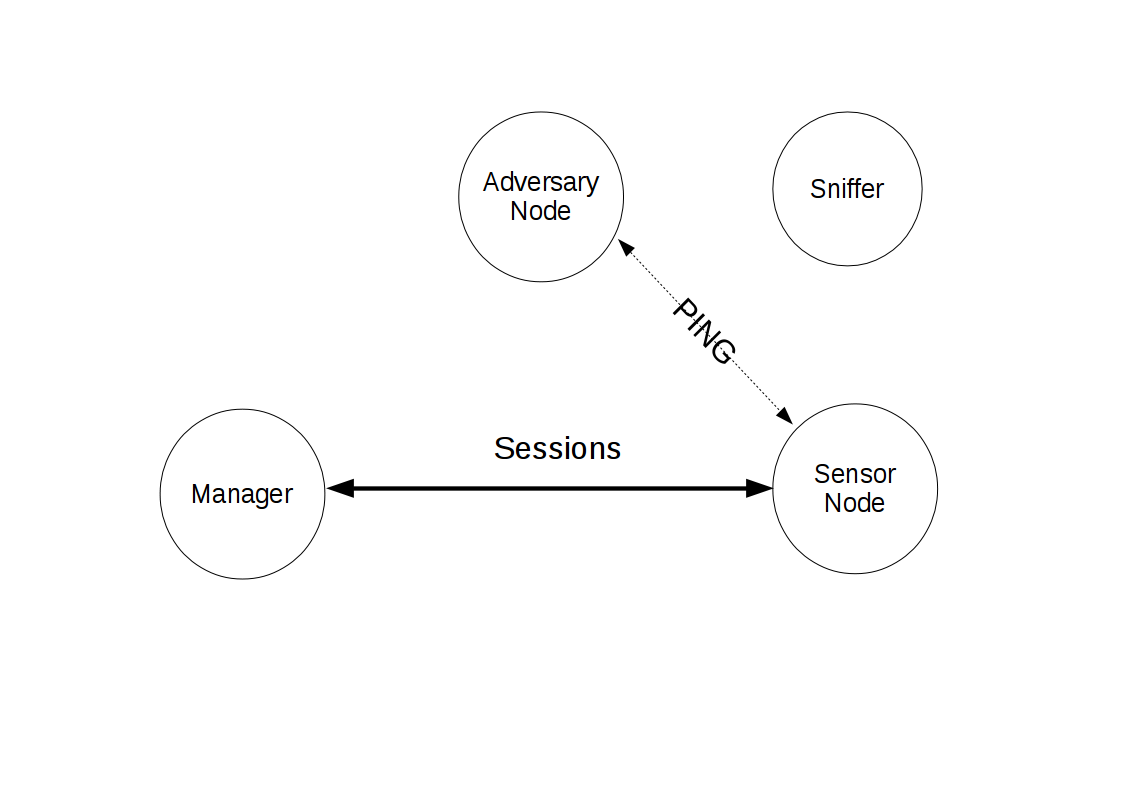
\includegraphics[width=0.8\textwidth]{fig/PINGLOAD_scenario.png}
	\caption{Scenario of PINGLOAD}
	\label{Fig: Scenario of PINGLOAD}
\end{figure*}

In this scenario, we assume the Manager engages with the target Sensor Node in Sessions. The Adversary Node is connected into the network and sends ICMP ECHO Requests (PING Request) to the Sensor Node. The Sensor Node, by default enabled by the Contiki system, replies with ICMP ECHO Responses (PING Respon. All packets are captured by the Adversary controlled Sniffer. \Cref{Fig: Time line of PINGLOAD} shows the time line of this scenario.

\begin{figure*}[h!]
	\center
	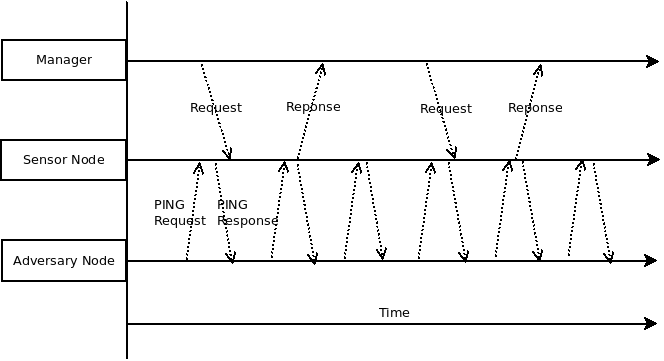
\includegraphics[width=0.8\textwidth]{fig/PINGLOAD_time.png}
	\caption{Time line of \Cref{Fig: Scenario of PINGLOAD}}
	\label{Fig: Time line of PINGLOAD}
\end{figure*}

\section{Phenomenon}

In our experiments, we realised that the latency between PING Request and PING Response varies according to the status of the Sensor Node. To be more specifically, the PING latency is apparently lower when the Sensor Node is not processing the Request sent by the Manager. The concept is shown in \Cref{Fig: Concept of PINGLOAD}. 

\begin{figure*}[h!]
	\center
	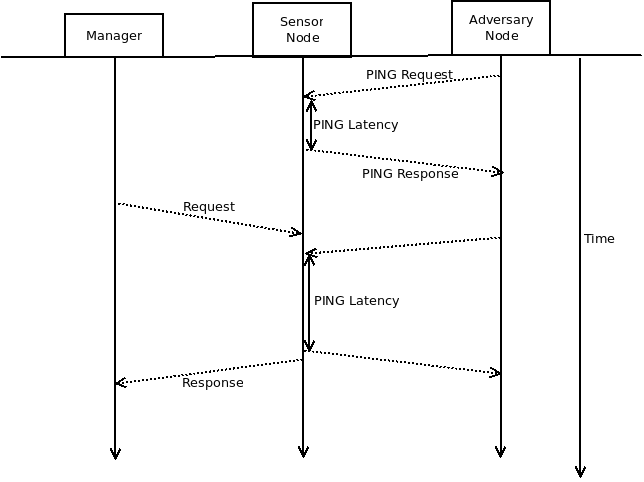
\includegraphics[width=0.8\textwidth]{fig/PINGLOAD_concept.png}
	\caption{Concept of PINGLOAD}
	\label{Fig: Concept of PINGLOAD}
\end{figure*}

This indicates that there is a potential leakage of the status of Sensor Node over the PING latency.

\section{Proof of Concept Experiment}

We set up a series of experiments to proof the potential of such side channel information leakage. The experiments are done in Cooja simulator with Wismote. The experiment WSN is set up as \Cref{Fig: Proof of concept experiment of PINGLOAD}.

\begin{figure*}
	\center
	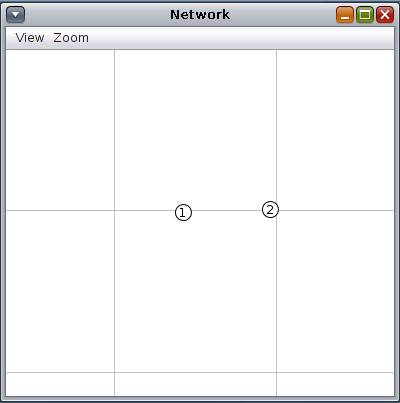
\includegraphics[width=0.5\textwidth]{fig/PINGLOAD_PoC.png}
	\caption{Proof of concept experiment of PINGLOAD. \textcirculed{1} is a border router and \textcirculed{2} is the target Sensor Node.}
	\label{Fig: Proof of concept experiment of PINGLOAD}
\end{figure*}

In this experiment, two procedure on our Linux host are used to simulate the Manager and the Adversary respectively. We argue this is equivalent to the settings of \Cref{Fig: Scenario of PINGLOAD} as we are evaluating the latency between PING Requests and PING Responses and thus the source of the PING Request is irrelevant in this experiment.

The target Sensor Node runs the dtlspingload application we explained in \Cref{Sec: Applications}. In this application, the Sensor Node establishes a DTLS connection with the Manager. Upon receiving a Request, the Sensor Node calls a ReadSensor() function to generate the data and replies that data to Manager, simulating a typical scenario in WSN. 

For this experiment, we defined two types of ReadSensor() functions. 

%
%\subsection{Hypothesis} \label{Sec: pingload hypothesis}
%A phenomenon we realised is that when a PING packet arrived while the target node is executing some payload, say reading a sensor or processing data, the PING RIs begin to vary comparing to a stable value when no payload is given to the sensor node. 
%
%\begin{example}
%\begin{figure}
%\centering
%{
%  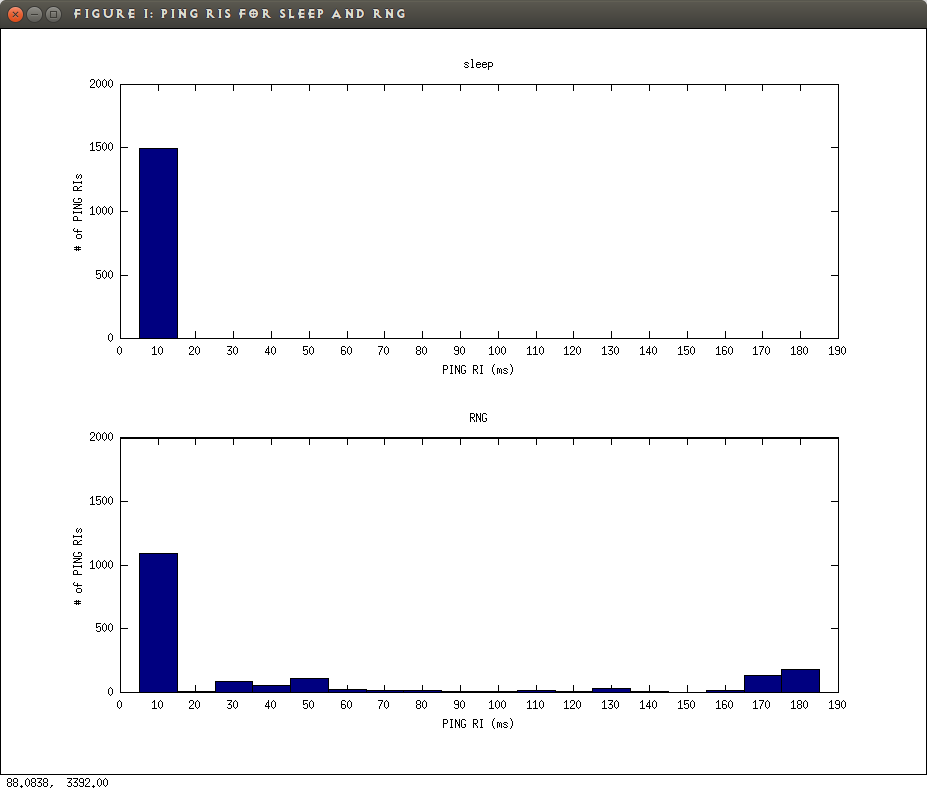
\includegraphics[width=1\textwidth]{fig/pingri.png}
%}
%\caption{An example of PING RIs with different payload}
%\label{Fig: PINGLOAD RIs}
%\end{figure}
%\Cref{Fig: PINGLOAD RIs} shows PING RIs collected in two experiments. In the upper half, the target node is constantly in asleep whilst in the lower half,  it occasionally receives a request which triggers the target to call RNG. We can see that the PING RI varies alongside the target is given some payload from this figure.
%\end{example}
%
%The data shown in \Cref{Fig: PINGLOAD RIs} suggests that the “plain”, that is without any interference, PING RI is 12 to 13 ms. Those variations of  shown in the lower half of \Cref{Fig: PINGLOAD RIs} is potentially caused by the payload on target.
%
%This result inspires us that the distributions of PING RIs might vary according to the payload on target and could possibly considered as a fingerprint to the target’s application. In other word, an adversary could possibly tell whether the target is running a specific application by looking at its PING RIs distribution.
%
%The attack then is strait forward:
%\begin{description}
%\item[Profile sleep RIs]: \hfill\\
%The PING RIs for a sleeping node of the same platform can be profiled by pinging a sleeping node. We denote the sleeping profile as $RI_{sleep}$. 
%
%\item[Fingerprint application]: \hfill\\
%The adversary collects PING RIs on a profiling node with known application. The profiling node needs to be of the same platform and executing the same code of the target’s. The profiled application fingerprint is a sample set of RIs, denotes as: $F_p=\{a_1, a_2, ... , a_n\}$ where $a_i$ is the RI of $i$th PING to the profiling node. 
%
%\item[Collect fingerprint of target]: \hfill\\
%The adversary then fingerprints the payload on the target in a similar way by pinging it. We denote the collected target sample set of RIs as: $F_t=\{b_1, b_2, ..., b_m\}$ where $b_j$ is the RI of $j$th PING to the target node.
%
%\item[Extract Featured RIs]: Since a node is usually in a sleep state, most of the PING RIs will hence results into $RI_{sleep}$. To improve the clarity of our fingerprint, we can remove them from the data sets and keep only the PING RIs those (seemingly) has been interfered by the payload. We denote the extracted RIs as \textbf{Featured RIs}:
%\begin{eqnarray*}
%F’_p = F_p - RI_{sleep} = \{x | x \in F_p,  x \notin RI_{sleep}\}\\
%F’_t = F_t - RI_{sleep} = \{x | x \in F_t,  x \notin RI_{sleep}\}
%\end{eqnarray*}
%
%Practically speaking, the PING protocol are designed to be responded immediately for diagnosis purpose; hence $RI_{sleep}$ usually has an extremely low variance and its mean is also much less than $F_p$ and $F_t$. Therefore we can ignore the error induced by wrongly removed packets.
%
%Using the Featured RIs not only provides a better vision of the fingerprint but also removes the error caused by different frequency of the target code being executed, as all the Featured RIs are  collected when the node is at a non-sleeping state. 
%
%\item[Estimate Distribution (Optional)]: \hfill\\
%We then estimate the distributions of $F’_p$ and $F’_t$, denote as $\mathbb{D}_p$ and $\mathbb{D}_t$. A naive method is to simply use their histograms. An example of such histograms are shown as \Cref{Fig: featuredri_rng}.
%
%\begin{figure}
%\center
%{
%	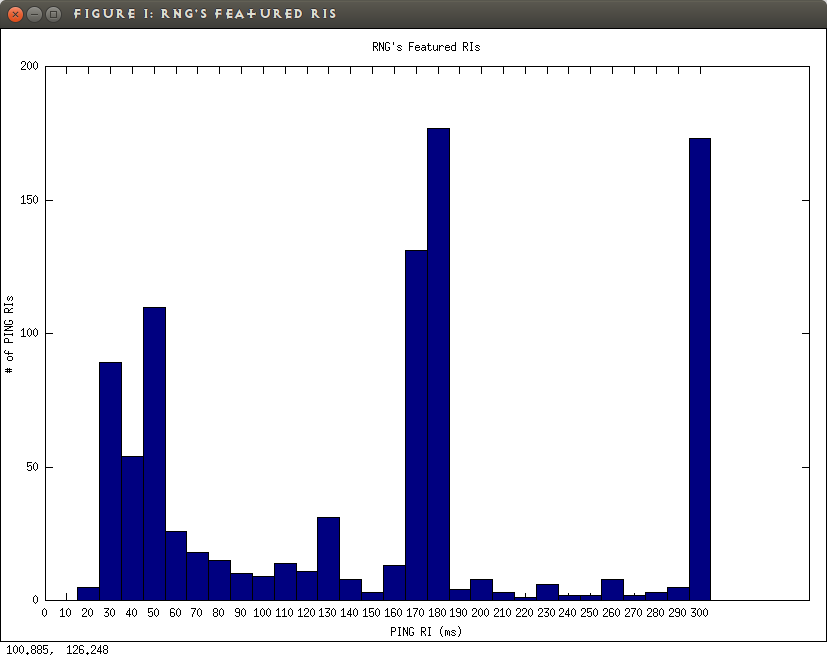
\includegraphics[width=0.49 \textwidth]{fig/featuredri_rng1.png}
%	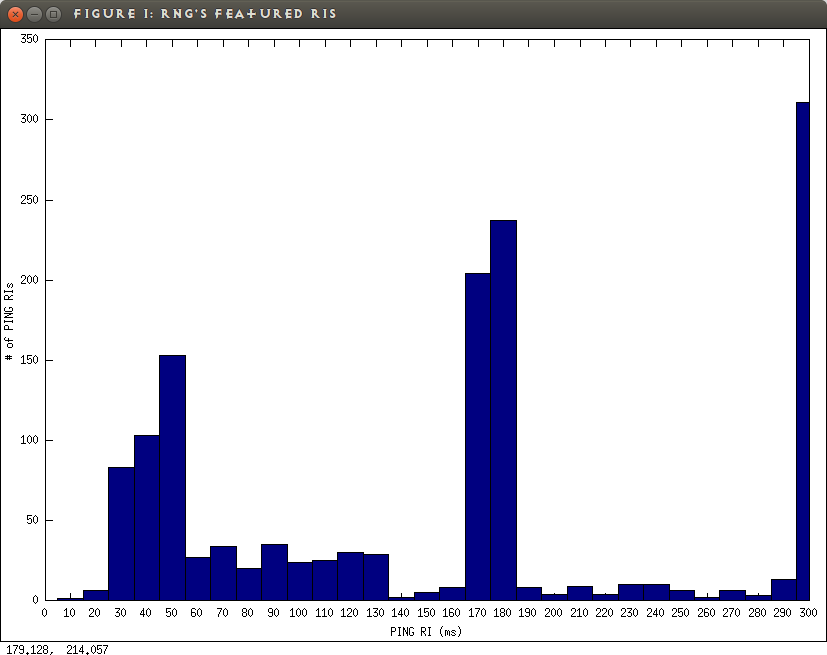
\includegraphics[width=0.49 \textwidth]{fig/featuredri_rng2.png}
%}
%\caption{Two examples of RNG’s Featured RIs histogram}
%\label{Fig: featuredri_rng}
%\end{figure}
%
%\item[Distinguish Distributions]: \hfill\\
%Finally we test whether $D_t$ and $D_p$ are the same distribution. A naive way is to compute the correlation of counts of the histograms. We conclude the target node is running the profiled application if $D_t$ and $D_p$ are the same distribution.
%\end{description}
%
%Practically speaking, the key point of Application Fingerprinting is to test whether the target’s Featured RIs is sampled from same distribution of the profiled one, i.e. whether $F’_t = F’_p$; therefore estimating their distribution might not be necessary for some statistical methods such as t-tests. However as we can see in \Cref{Fig: featuredri_rng}, PING RIs’ distribution are very unlikely to be normalised. Therefore a future work is to find a better distinguishing method than the current naive one.
%
%\subsection{Experiment Results}
%We tried our Application Fingerprinting attack in a Cooja simulated Wismote platform with different codes. \textbf{In conclusion, the fingerprint appears to be effective for certain circumstances but will tends to result into false positives as the profiled application and target application gets similar to each other.}
%
%To be more specifically, the target node execute some specific code upon receiving an application layer protocol request, similar to CoAP. Further more, all traffic are protected by DTLS with TLS\_PSK\_WITH\_AES\_128\_CCM\_8 ciphersuite. Both intervals of PINGs and the application request are set to some asynchronised value to avoid overflooding the target and to create a ‘more realistic’ simulation.
%
%Everything other than the examined code are the same for all experiments. Two samples are collected independently for each code to simulate a fingerprinting scenario. The histograms are clustered by 5ms from 0ms to 500ms.
%
%We examined two classes of codes:
%\begin{description}
%\item[RNG Calls]: \hfill\\
%The target node repeatedly calls RNG for $i$ times. We examined their Featured PING RI for different values of $i$. The reason for picking RNG is that on some platforms where a hardware RNG is provided, the call to it is expected to be similar to a call to a sensor reading which is actually an interrupt to the processor. Results are shown in \Cref{Tbl: pingload RNG}.
%
%\item[Arithmetic Operations]: \hfill\\
%The target node repeatedly does arithmetic operations, namely addition, multiplication and modular, on two randomly generated word size integers for 10000 times. This class is particularly interested from a cryptographic point of view as the number of arithmetic operations could potentially developed to key recovering attacks. Results are shown in \Cref{Tbl: pingload arth}.
%\end{description}
%
%
%
%\begin{table}
%\centering
%\begin{tabular}{|c|cccc}
%\hline
%\textit{\textbf{Correlations}} & \multicolumn{1}{c|}{i=50} & \multicolumn{1}{c|}{i=100} & \multicolumn{1}{c|}{i=2500} & \multicolumn{1}{c|}{i=5000} \\ \hline
%i=50                           & \textbf{0.988}            & 0.891                      & -0.014                      & -0.033                      \\ \cline{1-1}
%i=100                          & 0.891                     & \textbf{0.973}             & -0.025                      & -0.042                      \\ \cline{1-1}
%i=2500                         & -0.014                    & -0.025                     & \textbf{0.993}              & -0.035                      \\ \cline{1-1}
%i=5000                         & -0.033                    & -0.042                     & -0.035                      & \textbf{0.985}              \\ \cline{1-1}
%\end{tabular}
%\caption{Correlations for RNG}
%\label{Tbl: pingload RNG}
%\end{table}
%
%\begin{table}
%\centering
%\begin{tabular}{|c|ccc}
%\hline
%\textit{\textbf{Correlations}} & \multicolumn{1}{c|}{+} & \multicolumn{1}{c|}{*} & \multicolumn{1}{c|}{\%} \\ \hline
%+                              & \textbf{0.990}         & \textbf{0.990}         & \textbf{0.988}          \\ \cline{1-1}
%*                              & \textbf{0.990}         & \textbf{0.989}         & \textbf{0.985}          \\ \cline{1-1}
%\%                             & \textbf{0.988}         & \textbf{0.985}         & \textbf{0.984}          \\ \cline{1-1}
%\end{tabular}
%\caption{Correlations for word arithmetic operations}
%\label{Tbl: pingload arth}
%\end{table}
%
%\begin{table}[]
%\centering
%\begin{tabular}{|c|c|}
%\hline
%\textbf{\textit {Correlations}} & +     \\ \hline
%i=50         & 0.877 \\ \hline
%\end{tabular}
%\caption{Correlation for $i=50$ and addition}
%\label{Tbl: pingload rng arth}
%\end{table}
%
%We also computed the correlation for $i=50$ and addition, as shown in \Cref{Tbl: pingload rng arth}.
%
%The results suggests the following conjectures:
%\begin{enumerate}
%\item The results for RNG suggests that the fingerprinting is effective for this class of code, as the same code results into nearly perfect correlations ($\geq 0.95$).
%
%\item Even relatively slight changes can be detected, as we can see the correlation dropped to $0.891$ alongside 50 iterations of RNG calls (50 RNG calls take about 1.4ms).
%
%\item The results for arithmetic operations indicates that their  fingerprint are unlikely to be distinguishable. There are two potential causes we have considered:
%\begin{enumerate}
%\item The differences between these operations are too small to be detected.
%
%\item Experiment methodology error. Since the target node we used during the experiments call RNG twice upon each request to generate two operands whilst the word arithmetic operations have much lighter weigh comparing to RNG at magnitude level\footnote{A RNG call takes about 0.03ms where as an addition takes $\leq 2^{-20}$ms on the Wismote platform. }; thus the fingerprint is dominated by RNG rather than word arithmetic operations. As a result, we can see that a relatively high correlation can be observed between word addition and 50 RNG calls as shown in \Cref{Tbl: pingload rng arth}.
%\end{enumerate}
%\end{enumerate}
%
%\subsection{A General Hypothetical Model: Black Box Model}
%Although the experiments supports the hypothesis that the variation of PING RIs is relevant to the application, it is not yet clear which factor exactly caused the variations. 
%
%Therefore we instead suggest that this phenomenon is a result of multi factors, including:
%\begin{itemize} 
%\item Code being executed  and whether it is preemptive or non preemptive, 
%\item Memory usage, such as packet buffers, or 
%\item Any other hardware/software conditions.
%\end{itemize}
%It is difficult to verify these factors as many of them requires strict synchronisation between devices and the PING RIs are only showing statistical features.
%
%Therefore we propose the Black Box Model which we hope could support further research.
%
%\begin{definition}
%The \textbf{Black Box Model} models the target device as a stateful black box. A \textbf{state}, denotes as $\vec{S}=<\text{factor}_1, \text{factor}_2...>$, is an abstracted vector of multiple factors that could affect PING RIs, such as current code context or memory usage. $\mathbb{D}_{\vec{S}}$ is the distribution of PING RIs when the target node is at state $\vec{S}$.
%\end{definition}
%
%We can redefine a state by multiple mutually exclusive substates, $\vec{S}_1$, $\vec{S}_2$ etc. Each sub-state has its own PING RI distribution $\mathbb{D}_{\vec{S}_1}$, $\mathbb{D}_{\vec{S}_2}$ etc. The redefinition process can further more be done recursively.
%
%Notice that since each substate are mutually exclusive; thus:
%\begin{equation*}
%\forall x: Prob(RI = x | \vec{s}=\vec{S}) = \sum_{i=0}^{n}{\big( p_i*Prob(RI = x | \vec{s} = \vec{S}_i)\big)}
%\end{equation*}
%where $\vec{s}$ is the state at any moment, $p_i = Prob(\vec{s} = \vec{S_i})$ and $n$ is the number of substates of $\vec{S}$.
%
%Therefore $\mathbb{D}_{\vec{S}}$ is a linear combination of all distributions associated with all the substates of $\vec{S}$. Hence we can write
%\begin{equation} \label{Eq: pD}
%\mathbb{D}_{\vec{S}} = \sum_{i}^{n}{\big(p_i * \mathbb{D}_{\vec{S}_i} \big)}
%\end{equation}
%
%\begin{example} \label{Ex: Black Box Example}
%Take one of the RNG applications with $i = 5000$ in \Cref{Tbl: pingload RNG} for example. 
%
%We define the root state:
%\begin{equation*}
%\vec{S}_{root} = <\text{App}=\text{RNG}, i=5000>
%\end{equation*}
%
%Its associated PING RI distribution $\mathbb{D}_{\vec{S}_{root}}$ is approximated from the histogram shown in \Cref{Fig: s_root}.
%
%\begin{figure}
%\center
%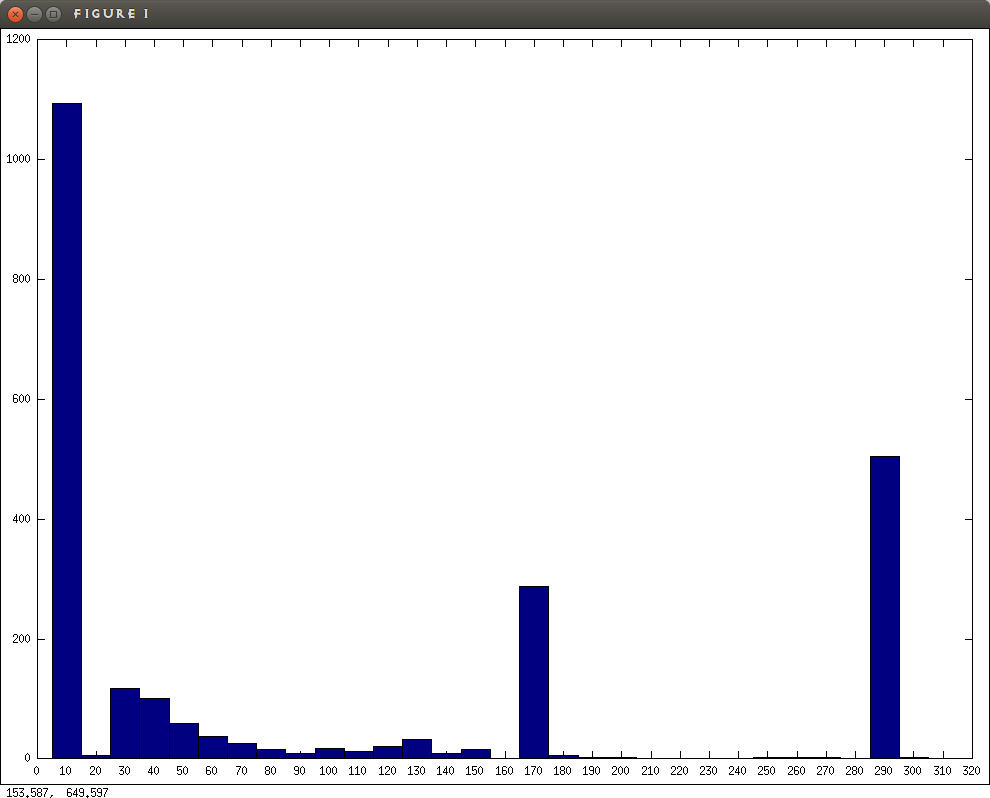
\includegraphics[width=0.5\textwidth]{fig/D_S.png}
%\caption{PING RIs of $\vec{S}_{root}$}
%\label{Fig: s_root}
%\end{figure}
%
%We then redefine $\vec{S}_{root}$ to two exclusive sub-states depends on whether the target is in a sleeping mode.
%\begin{eqnarray*}
%\vec{S}_{root} &&= \vec{S}_{sleep} + \vec{S}_{nonsleep} \\
%\vec{S}_{sleep} &&= <\text{App} = \text{RNG}, i = 5000, \text{Code} = \text{sleep}> \\
%\vec{S}_{nonsleep} &&= <\text{App} = \text{RNG}, i = 5000, \text{Code} \neq \text{sleep}>
%\end{eqnarray*}
%
%Since we know by experiment that the PING RIs are 12 to 13ms when the target is sleep; therefore we can actually approximate $\mathbb{D}_{\vec{S}_{sleep}}$ by filter out those RIs in $[12,13]$. Vice versa,  the distribution of Featured RIs can be viewed as $\mathbb{D}_{\vec{S}_{nonsleep}}$ since they are exactly the RIs filtered by the RIs of sleep. The histograms are shown in \Cref{Fig: s_sleep and s_nonsleep}.
%
%\begin{figure}
%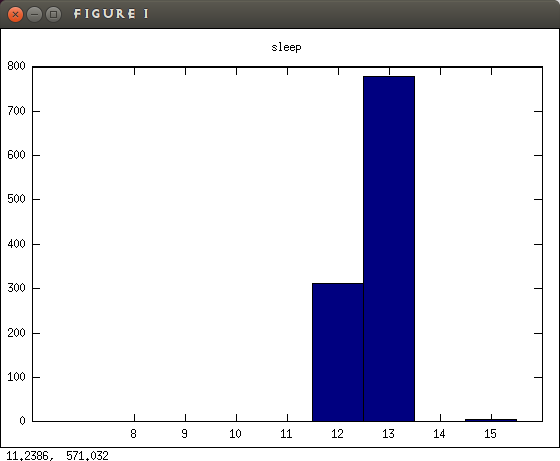
\includegraphics[width=0.5\textwidth]{fig/d_sleep.png}
%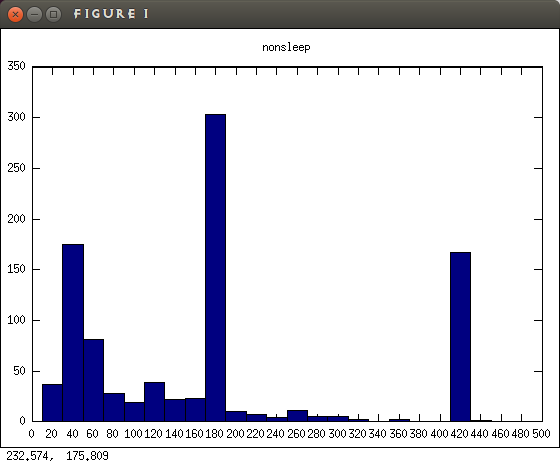
\includegraphics[width=0.5\textwidth]{fig/d_nonsleep.png}
%\caption{PING RIs of $\vec{S}_{sleep}$ and $\vec{S}_{nonsleep}$}
%\label{Fig: s_sleep and s_nonsleep}
%\end{figure}
%
%So we have
%\begin{equation} \label{Eq: sleep}
%\mathbb{D}_{\vec{S}_{main}} = p_0 \mathbb{D}_{\vec{S}_{sleep}} + p_1 \mathbb{D}_{\vec{S}_{nonsleep}}
%\end{equation}
%where $p_0$ and $p_1$ corresponds to the probability of the target being sleep and nonsleep.
%
%Solving \Cref{Eq: sleep} gives us roughly $p_0 = 0.538$ and $p_1 = 0.462$. Assuming the PING packets are received by the target randomly, we can estimate that the target is in sleep for $53.8\%$ and awake for $46.2\%$ of the time.
%
%Theoretically we can further redefine more sub-states, e.g.:
%\begin{eqnarray*}
%\vec{S}_{nonsleep} &&= \vec{S}_{RNG} + \vec{S}_{header} \\
%\vec{S}_{RNG} &&= <\text{App} = \text{RNG}, i = 5000, \text{Code} = \text{random\_rand()}> \\
%\vec{S}_{header} &&= <\text{App} = \text{RNG}, i = 5000, \text{Code} = \text{header processing}> 
%\end{eqnarray*}
%\end{example}
%
%Practically speaking, $p_i$ might be an interesting information to an  adversary as it reveals the internal state of the target which could lead to many information breach.  In practice, we might only want to approximate the solutions of $p_i$, which effectively reduces the problem of approximating \Cref{Eq: pD} to a knapsack problem\cite{knapsack}. In most cases obtaining $\mathbb{D}_{\vec{S}_i}$ is difficult as it is hard to determine the exactly the state of target sensor node at an exact moment, as in \Cref{Ex: Black Box Example}. We leave this problem to future research.
